\documentclass{article}
\usepackage{tikz}
\usetikzlibrary{arrows.meta}

\begin{document}

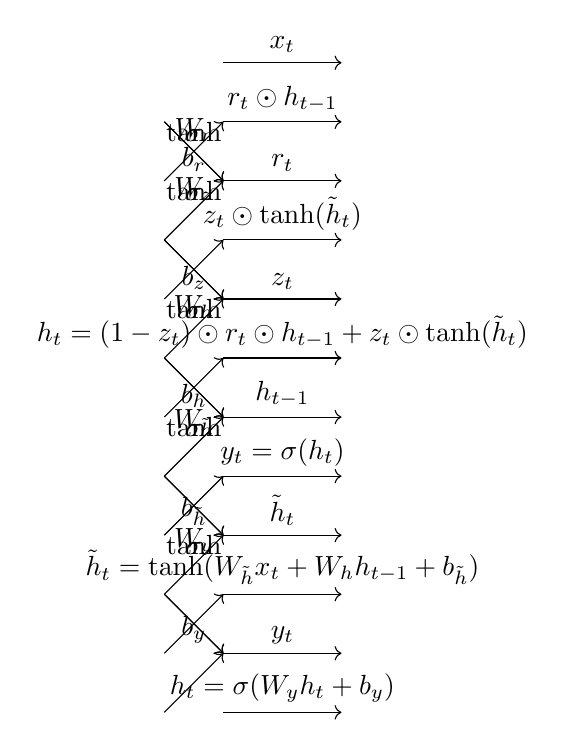
\begin{tikzpicture}[scale=1.5]
    % Input gate
    \draw[->] (-0.5, 0) -- (0.5, 0);
    \node at (0, 0) [above] {$x_t$};
    
    % Reset gate
    \draw[->] (-0.5, -1) -- (0.5, -1);
    \node at (0, -1) [above] {$r_t$};
    
    % Update gate
    \draw[->] (-0.5, -2) -- (0.5, -2);
    \node at (0, -2) [above] {$z_t$};
    
    % Hidden state
    \draw[->] (-0.5, -3) -- (0.5, -3);
    \node at (0, -3) [above] {$h_{t-1}$};
    
    % Candidate hidden state
    \draw[->] (-0.5, -4) -- (0.5, -4);
    \node at (0, -4) [above] {$\tilde{h}_t$};
    
    % Output gate
    \draw[->] (-0.5, -5) -- (0.5, -5);
    \node at (0, -5) [above] {$y_t$};
    
    % Gates weights
    \draw[->] (-1, -1) -- (-0.5, -0.5);
    \node at (-0.75, -0.75) [above] {$W_r$};
    
    \draw[->] (-1, -2) -- (-0.5, -1.5);
    \node at (-0.75, -1.25) [above] {$W_z$};
    
    \draw[->] (-1, -3) -- (-0.5, -2.5);
    \node at (-0.75, -2.25) [above] {$W_h$};
    
    \draw[->] (-1, -4) -- (-0.5, -3.5);
    \node at (-0.75, -3.25) [above] {$W_{\tilde{h}}$};
    
    \draw[->] (-1, -5) -- (-0.5, -4.5);
    \node at (-0.75, -4.25) [above] {$W_y$};
    
    % Gates biases
    \draw[->] (-1, -1.5) -- (-0.5, -1);
    \node at (-0.75, -1) [above] {$b_r$};
    
    \draw[->] (-1, -2.5) -- (-0.5, -2);
    \node at (-0.75, -2) [above] {$b_z$};
    
    \draw[->] (-1, -3.5) -- (-0.5, -3);
    \node at (-0.75, -3) [above] {$b_h$};
    
    \draw[->] (-1, -4.5) -- (-0.5, -4);
    \node at (-0.75, -4) [above] {$b_{\tilde{h}}$};
    
    \draw[->] (-1, -5.5) -- (-0.5, -5);
    \node at (-0.75, -5) [above] {$b_y$};
    
    % Gates activation functions
    \draw[->] (-1, -0.5) -- (-0.5, -1);
    \node at (-0.75, -0.75) [above] {$\sigma$};
    
    \draw[->] (-1, -1.5) -- (-0.5, -2);
    \node at (-0.75, -1.25) [above] {$\sigma$};
    
    \draw[->] (-1, -2.5) -- (-0.5, -3);
    \node at (-0.75, -2.25) [above] {$\sigma$};
    
    \draw[->] (-1, -3.5) -- (-0.5, -4);
    \node at (-0.75, -3.25) [above] {$\sigma$};
    
    \draw[->] (-1, -4.5) -- (-0.5, -5);
    \node at (-0.75, -4.25) [above] {$\sigma$};
    
    % Gates non-linearities
    \draw[->] (-1, -0.5) -- (-0.5, -1);
    \node at (-0.75, -0.75) [above] {$\tanh$};
    
    \draw[->] (-1, -1.5) -- (-0.5, -2);
    \node at (-0.75, -1.25) [above] {$\tanh$};
    
    \draw[->] (-1, -2.5) -- (-0.5, -3);
    \node at (-0.75, -2.25) [above] {$\tanh$};
    
    \draw[->] (-1, -3.5) -- (-0.5, -4);
    \node at (-0.75, -3.25) [above] {$\tanh$};
    
    \draw[->] (-1, -4.5) -- (-0.5, -5);
    \node at (-0.75, -4.25) [above] {$\tanh$};
    
    % Gates outputs
    \draw[->] (-0.5, -0.5) -- (0.5, -0.5);
    \node at (0, -0.5) [above] {$r_t \odot h_{t-1}$};
    
    \draw[->] (-0.5, -1.5) -- (0.5, -1.5);
    \node at (0, -1.5) [above] {$z_t \odot \tanh(\tilde{h}_t)$};
    
    \draw[->] (-0.5, -2.5) -- (0.5, -2.5);
    \node at (0, -2.5) [above] {$h_t = (1-z_t) \odot r_t \odot h_{t-1} + z_t \odot \tanh(\tilde{h}_t)$};
    
    \draw[->] (-0.5, -3.5) -- (0.5, -3.5);
    \node at (0, -3.5) [above] {$y_t = \sigma(h_t)$};
    
    \draw[->] (-0.5, -4.5) -- (0.5, -4.5);
    \node at (0, -4.5) [above] {$\tilde{h}_t = \tanh(W_{\tilde{h}} x_t + W_h h_{t-1} + b_{\tilde{h}})$};
    
    \draw[->] (-0.5, -5.5) -- (0.5, -5.5);
    \node at (0, -5.5) [above] {$h_t = \sigma(W_y h_t + b_y)$};
\end{tikzpicture}

\end{document}